%======================================================================
\section{Sensitivity and robustness}\label{app:sens}
%======================================================================

This appendix collects the sensitivity analyses referred to in Section~\ref{sec:results}. They use the stored
per-split results and the per-epoch records of the search, and they train no model.

\subsection{Size of the searched space}\label{sec:res-budget}

The searched spaces differ in size, from 6 configurations for several KuaiRand-Pure and KuaiRec baselines to 324 for
the QP family on Coat. To measure how much this matters, we drew 1,000 random subsets of $k_\mathrm{min}$
configurations for each comparison and counted how often its sign changed (Table~\ref{tab:T7}). Flips are common for
comparisons whose effects are near zero. The QP family against LightGCN-p changes sign in $35.3\%$ of the subsets on
Coat and $30.9\%$ on KuaiRec. The largest instability is DRUP against DR-JL on KuaiRec. At $k_\mathrm{min}=6$, $78.4\%$
of the subsets flip the sign, and the split-mean difference at matched budget is $-14.90$, while the full-search-space
per-user difference is $+4.38$ [2.21]. DRUP is training-free but searches 384 configurations on KuaiRec, against 6 for
DR-JL, so its advantage over DR-JL depends on the budget granted to each method. The matched-budget values in
Table~\ref{tab:T5} are split means and carry no test.

\begin{table}[t]
\centering
\footnotesize
\caption{Sensitivity of the primary conclusions to evaluation choices (A1, A2). A check mark means the sign of the difference (and, for Main, significance at $p_\mathrm{Holm}<0.05$) survives the choice; the value is the difference $\times10^{3}$ under that choice. Main: per-user difference. Oracle, configuration-oracle and matched-budget columns: split-mean difference, compared in sign with the split-mean validation-selected difference.}
\label{tab:T7}
\resizebox{\textwidth}{!}{%
\begin{tabular}{lllllllrrlll}
\toprule
Dataset & Fam. & Comparison & Main (Holm) & Test oracle & Config.\ oracle & Matched $k$ & $k_\mathrm{min}$ & Flip share & Seeds & NB & Alt.\ metric \\
\midrule
Coat & P1 & DR-LightGCN -- LightGCN & $\times$ -0.65 & $\checkmark$ +1.23 & $\times$ -6.63 & $\checkmark$ +4.11 & 54 & 0.0\% & n/a & $\times$ & $\times$ \\
Coat & P2 & iALS-p (add prior) -- iALS & $\times$ +16.82 & $\checkmark$ +31.66 & $\checkmark$ +21.23 & $\checkmark$ +16.12 & 24 & 0.0\% & n/a & $\times$ & $\checkmark$ \\
Coat & P2 & LightGCN-p (add prior) -- LightGCN & $\checkmark$ +31.98 & $\checkmark$ +27.74 & $\checkmark$ +28.27 & $\checkmark$ +34.12 & 54 & 0.0\% & n/a & $\times$ & $\checkmark$ \\
Coat & P3 & QP family (pooled) -- LightGCN-p (add prior) & $\times$ +0.05 & $\times$ +2.17 & $\times$ +1.42 & $\checkmark$ -0.36 & 108 & 35.3\% & n/a & $\times$ & $\times$ \\
Coat & P3 & DR-iALS -- iALS-p (add prior) & $\times$ -10.22 & $\checkmark$ -24.87 & $\checkmark$ -13.87 & $\checkmark$ -11.21 & 48 & 0.0\% & n/a & $\times$ & $\checkmark$ \\
Yahoo & P1 & r-AdjNorm -- LightGCN & $\checkmark$ +4.10 & $\checkmark$ +2.35 & $\checkmark$ +0.57 & $\checkmark$ +2.87 & 36 & 2.4\% & $\checkmark$ & $\times$ & $\checkmark$ \\
Yahoo & P2 & LightGCN-p (add prior) -- LightGCN & $\times$ -1.43 & $\checkmark$ -0.07 & $\checkmark$ -1.11 & $\checkmark$ -2.16 & 24 & 0.0\% & n/a & $\times$ & $\checkmark$ \\
KuaiRand & P1 & r-AdjNorm -- LightGCN & $\checkmark$ +1.99 & $\checkmark$ +1.76 & $\checkmark$ +1.80 & $\checkmark$ +1.23 & 6 & 9.4\% & $\checkmark$ & $\times$ & $\checkmark$ \\
KuaiRand & P2 & LightGCN-p (add prior) -- LightGCN & $\times$ -0.81 & $\checkmark$ -0.03 & $\checkmark$ -0.84 & $\checkmark$ -0.79 & 6 & 7.1\% & n/a & $\times$ & $\checkmark$ \\
KuaiRec & P1 & DR-LightGCN -- LightGCN & $\checkmark$ +13.17 & $\checkmark$ +14.69 & $\checkmark$ +12.44 & $\checkmark$ +12.97 & 6 & 0.0\% & n/a & $\times$ & $\times$ \\
KuaiRec & P2 & LightGCN-p (add prior) -- LightGCN & $\checkmark$ +21.22 & $\checkmark$ +20.02 & $\checkmark$ +20.00 & $\checkmark$ +20.25 & 24 & 0.0\% & n/a & $\checkmark$ & $\checkmark$ \\
KuaiRec & P2 & iALS-p (add prior) -- iALS & $\checkmark$ +14.74 & $\checkmark$ +14.00 & $\checkmark$ +14.00 & $\checkmark$ +16.89 & 8 & 0.0\% & n/a & $\checkmark$ & $\checkmark$ \\
KuaiRec & P3 & QP family (pooled) -- LightGCN-p (add prior) & $\times$ -0.32 & $\times$ +0.32 & $\times$ +0.46 & $\checkmark$ -0.12 & 24 & 30.9\% & n/a & $\times$ & $\checkmark$ \\
KuaiRec & P4 & DRUP -- DR-JL & $\checkmark$ +4.38 & $\checkmark$ +5.48 & $\checkmark$ +5.45 & $\times$ -14.90 & 6 & 78.4\% & n/a & $\times$ & $\checkmark$ \\
\bottomrule
\end{tabular}}
\par\smallskip\raggedright\footnotesize Flip share: fraction of 1,000 random subgrids of $k_\mathrm{min}$ configurations per method whose sign differs from the full grid. Alt.\ metric: nDCG@10 (Coat, Yahoo), nDCG@20 (KuaiRand), nDCG@50 (KuaiRec), on the stored selections.
\end{table}


\subsection{Weighting unit, metric and seeds}

The weighting unit can also change a sign. For DR-LightGCN against LightGCN on Coat, the split-mean difference at
matched budget ($k=54$) is $+4.11$, while the per-user paired difference is $-0.65$ [30.16]. Every test in this paper
uses the per-user unit. Changing the metric changes 3 of the 14 pairwise conclusions in Table~\ref{tab:T7}: the Coat
comparisons of DR-LightGCN with LightGCN and of the QP family with LightGCN-p, and the KuaiRec comparison of
DR-LightGCN with LightGCN. The alternative metric is nDCG@10 on Coat and Yahoo! R3, nDCG@20 on KuaiRand-Pure and
nDCG@50 on KuaiRec. Of the 14 comparisons in Table~\ref{tab:T7}, 7 are significant at $p_\mathrm{Holm}<0.05$ in the
main run. Over all 14 comparisons, the sign survives the per-split test oracle in 12, the configuration-level oracle in
11, the matched budget in 13 and the alternative metric in 11.

Retraining the selected configurations with seeds 1 to 3 changes two main-run conclusions (the seeds column of
Table~\ref{tab:T5}). These comparisons are descriptive, because the two baselines of each dataset were chosen on test
data. On Coat, \qp{} against iALS is $+20.02$ [19.74] in the main run ($p_\mathrm{Holm}=0.0469$, nominal, in a family of
eight baselines). Over seeds 1 to 3 the difference is $+3.39$ [20.70] ($p_\mathrm{Holm}=0.747$, in a family of two),
which is not significant. On KuaiRec the main-run deficits of \qp{} against DR-JL and MRDR, $-4.56$ [2.24] and $-4.34$
[2.16], shrink over seeds 1 to 3 to $-1.03$ [1.64] ($p_\mathrm{Holm}=0.2213$) and $-1.56$ [1.47] ($p_\mathrm{Holm}=0.0760$).
On Yahoo! R3 and KuaiRand-Pure the \qp{} family exceeds r-AdjNorm by $+14.76$ [5.23] and by $+2.31$ [1.23] over seeds 1
to 3; these seed comparisons are descriptive and carry no significance claim. The seed-to-seed standard deviation of
\qp{} on Coat ($0.0049$, ddof 0) is larger than that of iALS ($0.0029$), so the main-run Coat result is a single-run
result.

\subsection{Bootstrap ranks}

\begin{figure}[htbp]
\centering
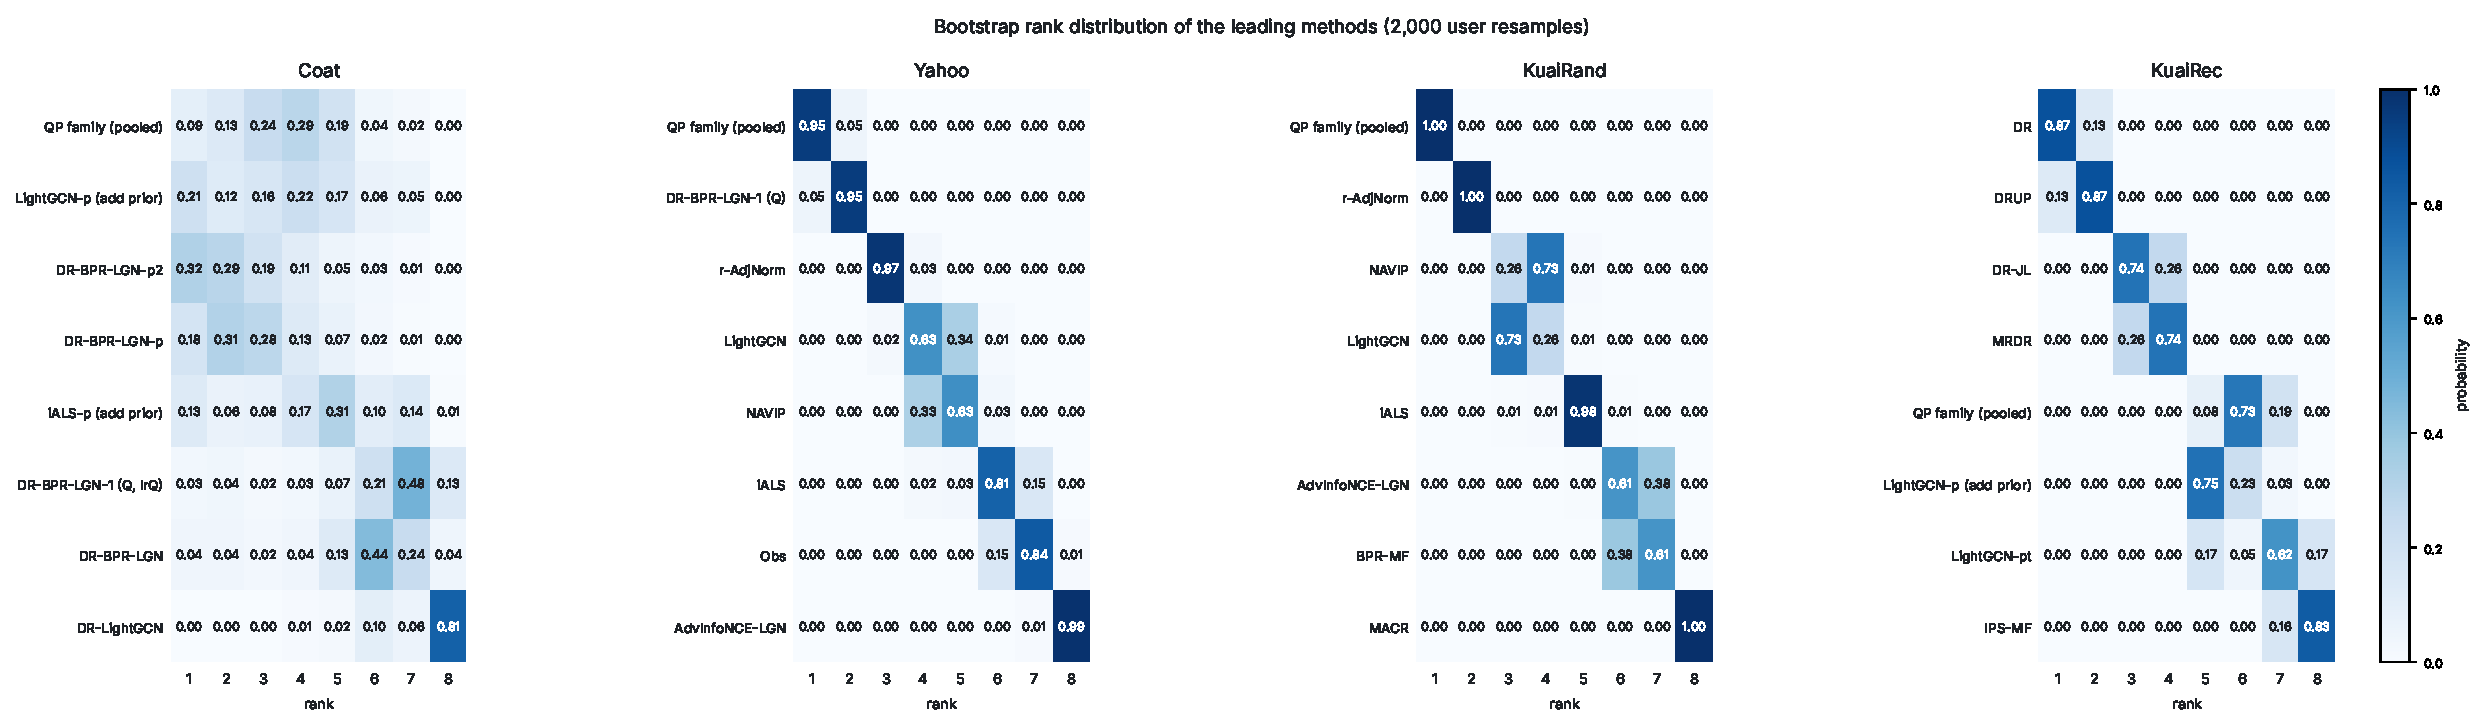
\includegraphics[width=\linewidth]{figs/rank_distribution}
\caption{Bootstrap rank distributions over 2,000 user resamples. For each dataset the rows are the eight methods with the
highest mean validation score, excluding control rows, and the columns are the rank by mean test score (1 is best). On
Coat the splits are resampled together with the users. Each cell gives the probability of that rank.}
\label{fig:rank}
\end{figure}

The bootstrap ranks (Figure~\ref{fig:rank}) show how stable the leader is. On Yahoo! R3 the QP family ranks first in
95.0\% of user resamples, and on KuaiRand-Pure in 99.8\%. On KuaiRec, DR and DRUP have the same mean score (0.6378) and
exchange first place, with probabilities 0.873 and 0.127. The bootstrap therefore cannot separate them. On Coat no
method is a stable leader. The most frequent first place is DR-BPR-LGN-p2, with probability 0.319, and the QP family
ranks first with probability 0.090.

\subsection{Two checks on the prior inputs}

Coat's shipped propensities were estimated by the dataset authors from the uniform sample, so the prior rows were
refitted with the estimator used on the other three datasets (Table~\ref{tab:T10}). The estimated-minus-shipped
difference is $+2.63$ [5.27] for iALS-p and $+1.64$ [10.30] for LightGCN-p, and the imputation alone changes by $-1.14$
[7.26]. None is significant. The gain over the no-prior reference remains as a point estimate: $+19.44$ [18.66] for
iALS-p ($p_\mathrm{Holm}=0.330$, not significant) and $+33.62$ [16.72] for LightGCN-p. The estimated-propensity run of
LightGCN was not carried out, and the other propensity-based Coat rows were not refitted.

\begin{table}[t]
\centering
\footnotesize
\caption{Coat with estimated propensities (X2): --prop pop versus the shipped propensities.}
\label{tab:T10}
\resizebox{\textwidth}{!}{%
\begin{tabular}{llrrrrr}
\toprule
Method & Propensities & nDCG (mean $\pm$ sd) & $\Delta$ vs no-prior $\times10^{3}$ [CI] & $p_\mathrm{Holm}$ & Estimated $-$ shipped $\times10^{3}$ [CI] & $p_\mathrm{Holm}$ \\
\midrule
iALS-p & shipped & 0.5984 $\pm$ 0.0128 & +16.82 [18.04] & 0.380 & -- & -- \\
iALS-p & estimated & 0.6009 $\pm$ 0.0120 & +19.44 [18.66] & 0.330 & +2.63 [5.27] & 1.000 \\
LightGCN-p & shipped & 0.6020 $\pm$ 0.0156 & +31.98 [20.65] & 0.023 & -- & -- \\
LightGCN-p & estimated & 0.6025 $\pm$ 0.0154 & +33.62 [16.72] & $<$0.001 & +1.64 [10.30] & 1.000 \\
iALS-wide & shipped & 0.5869 $\pm$ 0.0124 & +7.39 [7.52] & 0.380 & -- & -- \\
iALS-wide & estimated & 0.5869 $\pm$ 0.0124 & +7.39 [7.52] & 0.380 & 0 (identical) & 1 \\
imputation alone (add) & shipped & 0.5585 $\pm$ 0.0105 & -- & -- & -- & -- \\
imputation alone (add) & estimated & 0.5573 $\pm$ 0.0097 & -- & -- & -1.14 [7.26] & 1.000 \\
iALS (no prior) & shipped & 0.5812 $\pm$ 0.0107 & -- & -- & -- & -- \\
LightGCN (no prior) & shipped & 0.5683 $\pm$ 0.0139 & -- & -- & -- & -- \\
\bottomrule
\end{tabular}}
\par\smallskip\raggedright\footnotesize The no-prior reference of each learner is the stored run. Plain iALS and LightGCN do not read the propensities (only NAVIP does), so the shipped no-prior run is the reference for the estimated rows. LightGCN with estimated propensities was not run. $p_\mathrm{Holm}$ over the tests of this table.
\end{table}


The stored iALS search space selects its largest value of the confidence weight $\alpha$ (30) in all 10 splits, and the
wider search space of Table~\ref{tab:T11} selects its largest value (1000) in four splits. The stored search space is
therefore bounded at its edge, and the wider one is not exhausted. Over the stored iALS, the wider search space gives
$+12.92$ [8.01] ($p_\mathrm{Holm}=0.003$), against $+16.82$ [18.04] for the offset model over the same stored iALS. The
wider search space is not significantly different from iALS-p ($-3.90$ [15.99], $p_\mathrm{Holm}=0.631$). The two
differences cannot be separated: the wider search space has 32 configurations against 90 for iALS-p.

\begin{table}[t]
\centering
\footnotesize
\caption{Coat iALS with the wider grid (X4) against the stored iALS and iALS-p.}
\label{tab:T11}
\resizebox{\textwidth}{!}{%
\begin{tabular}{llrrrrrrl}
\toprule
Model & Grid & Cfg & nDCG (mean $\pm$ sd) & $\Delta$ vs iALS $\times10^{3}$ [CI] & $p_\mathrm{Holm}$ & $\Delta$ vs iALS-p $\times10^{3}$ [CI] & $p_\mathrm{Holm}$ & Selected values (number of splits) \\
\midrule
iALS (stored) & alpha \{3,10,30\} x reg \{1,10,100,1000\} x dim \{32,64\} & 24 & 0.5812 $\pm$ 0.0107 & ref. & -- & -- & -- & alpha 30:10; reg 100:10 \\
iALS-wide (v5 grid) & alpha \{10,30,100\} x reg \{10,100,300\} x dim \{32,64\} & 18 & 0.5869 $\pm$ 0.0124 & -- & -- & -- & -- & alpha 30:1, 100:9; reg 100:4, 300:6 \\
iALS-wide2 (X4 grid) & alpha \{30,100,300,1000\} x reg \{10,100,300,1000\} x dim \{32,64\} & 32 & 0.5922 $\pm$ 0.0150 & +12.92 [8.01] & 0.003 & -3.90 [15.99] & 0.631 & alpha 30:1, 100:4, 300:1, 1000:4; reg 100:2, 300:3, 1000:5 \\
iALS-p add (stored) & alpha \{10,30,100\} x reg \{10,100,300\} x pbeta \{0.1,0.2,0.3,0.5,1\} x dim \{32,64\} & 90 & 0.5984 $\pm$ 0.0128 & -- & -- & -- & -- & alpha 30:2, 100:8; reg 100:4, 300:6 \\
\bottomrule
\end{tabular}}
\par\smallskip\raggedright\footnotesize $\Delta$ = per-user paired difference (mean over the 10 splits), $\times10^{3}$, [half-width of the 95\% CI]. $p_\mathrm{Holm}$ over the two comparisons of iALS-wide2. Selected values are counted over the 10 splits.
\end{table}

